\def\mychapter{IX}
%this chapter was revised

\ifdefined\book
\else
\documentclass[11pt,oneside]{amsbook}
\usepackage[backend=biber, citestyle=authoryear]{biblatex}
\usepackage{mathpazo}
\usepackage{graphicx}
\usepackage{amsmath}
\usepackage{tikz}
\usetikzlibrary{arrows}
%\usepackage{titlesec}
\addbibresource{bibliography.bib}
\newcommand\posscite[1]{\citeauthor{#1}'s (\citeyear{#1})}
\newcommand\plural[1]{#1\mathrm{s}}
%\def\posscitewithextra[#1]#2{\citename{#2}'s (\citeyear{#2}, #1)}

%\newcounter{subsubsubsection}[subsubsection]
%\renewcommand\thesubsubsubsection{\thesubsubsection.\arabic{subsubsubsection}}
%\titleformat{\subsubsubsection}
%  {\normalfont\normalsize\bfseries}{\thesubsubsubsection}{1em}{}
%\titlespacing*{\subsubsubsection}
%{0pt}{3.25ex plus 1ex minus .2ex}{1.5ex plus .2ex}

\ifdefined\book
\renewcommand{\thechapter}{\Roman{chapter}}
\else
\renewcommand{\thechapter}{\mychapter}
\fi

\linespread{1.7}
\usepackage[margin=1.25in]{geometry}
\sloppy
\makeatletter
%% TODO: This is a cheat. It's supposed to be {paragraph}{4}, and that's 
%% what it is in amsbook.cls, but then it fails.
\def\paragraph{\@startsection{paragraph}{3}%
  \normalparindent\z@{-\fontdimen2\font}%
  \normalfont}
\def\subsubsubsection{\paragraph}
\makeatother

\def\smalltick{0.15cm}
\def\bigtick{0.3cm}
\def\pointcircle{0.08cm}
\def\causalnode{0.35cm}

\hyphenation{dia-chro-nic}

%\usepackage[utf8]{inputenc} % set input encoding (not needed with XeLaTeX)
\usepackage{amssymb}
\usepackage{mathtools}
\usepackage{enumitem}
\usepackage{amsthm}
\usepackage{physics}
%\usepackage{ntheorem}
\usepackage{chngcntr}
\counterwithin{figure}{section}

\makeatletter
% \def\@endtheorem{\endtrivlist\@endpefalse }% OLD
\def\@endtheorem{\endtrivlist}%

\setlist[description]{font=\normalfont\scshape}

\catcode`\|=\active\def|{\mid}
\DeclarePairedDelimiter{\ceil}{\lceil}{\rceil}
\DeclarePairedDelimiter{\floor}{\lfloor}{\rfloor}
\newcommand{\Subj}{\mathbin{\raisebox{.15ex}{$\scriptscriptstyle{\Box}$}\kern-.425em\rightarrow}}
\def\Existence{E!}
\def\Believes{\operatorname{Believes}}
\def\True{\operatorname{True}}
\def\Perfection{\operatorname{Perfection}}
\def\ext{\operatorname{Ext}}
\def\Iff{\leftrightarrow}
\def\Implies{\rightarrow}
\def\Entails{\Rightarrow}
\def\Cov{\operatorname{Cov}}
\def\Equiv{\Leftrightarrow}
\def\Form{\operatorname{Form}}
\def\Informs{\operatorname{Informs}}
\def\technical{$\star$}
\def\vtechnical{$\star\star$}
\def\power{\wp}
\def\Nec{\Box}
\def\Poss{\Diamond}
\def\Prop#1{$\langle$#1$\rangle$}
\def\R{\mathbb R}
\def\N{\mathbb N}
\def\tele{tel\={e}}
\makeatletter
\newtheoremstyle{indented}{3pt}{3pt}{\addtolength{\leftskip}{4.5em}}{-2.5em}{\sc}{.}{.5em}{}
\def\Principle#1#2#3{\theoremstyle{indented}\newtheorem*{principle}{#2}\begin{principle}\def\@currentlabel{#2}\label{#1}#3\end{principle}\let\principle\undefined}
\makeatother
\def\pref#1{{\sc\ref{#1}}}
\def\enum#1{\resume{enumerate}\item #1\end{enumerate}}
\def\ditem#1#2{\begin{enumerate}[resume]\item \label{\mychapter:#1} #2\end{enumerate}}
\def\nitem#1#2{\begin{description}\item[#1\label{\mychapter:#1}] #2\end{description}}
\def\bref#1{\ref{\mychapter:#1}}
\def\dref#1{(\ref{\mychapter:#1})}
\def\drefglobal#1{(\ref{#1})}
\usepackage{graphicx} % support the \includegraphics command and options
\usepackage{array} % for better arrays (eg matrices) in maths
\def\Not{\operatorname{\sim}}
\def\St{\operatorname{St}}
\def\num{\operatorname{num}}
\def\And{\mathrel{\&}}
\def\Or{\vee}
\def\BigOr{\bigvee}
\def\<{\langle}
\def\>{\rangle}
\def\union{\cup}
\def\nleq{\not\le}
\def\N{\mathbb N}
\def\R{\mathbb R}
\def\C{\mathbb C}
\def\Powerset{\mathcal P}
\def\star#1{{}^*#1}
\def\hN{\star{\N}}
\def\hR{\star{\R}}
\def\Z{\mathbb Z}
\def\Power{\mathcal P}
\def\Implies{\rightarrow}
\def\True{\operatorname{True}}
\def\Socrates{\mathrm{Socrates}}
\def\actual{@}
\def\Law{\operatorname{Law}}
\def\Chance{\operatorname{Chance}}
\def\Var{\operatorname{Var}}

\def\H2O{H${}_2$O}

\def\scr{\mathcal}
\def\e{\varepsilon}
\def\eps{\varepsilon}
\newtheorem{lem}{Lemma}
\newtheorem{prp}{Proposition}
\newtheorem*{theorem}{Theorem}
\newtheorem{corollary}{Corollary}
\newtheorem{cond}{Condition}

\renewcommand\thechapter{\Roman{chapter}}

\def\chaptertail{\ifdefined\book\else\end{document}\fi}
 

\title{Infinity, Causation and Paradox}
\author{Alexander R. Pruss}
%\date{} % Activate to display a given date or no date (if empty),
         % otherwise the current date is printed

\begin{document}
\setcounter{secnumdepth}{3}
\setcounter{tocdepth}{4}

\end{document}
\fi

\restartlist{enumerate}

\chapter{Metaphysics}\label{ch:metaphysics}
\section{Composition}
Intuitively, your parts compose a whole, namely you. On the other hand,
if you choose exactly one atom from every star in every galaxy in the universe,
intuitively these scattered atoms do not make up any whole.

Yet it seems that one could produce a continuous series of worlds, adding, subtracting or moving 
one particle at a time, where the first item in the series consists of the scattered
atoms in different stars and the last item consists of you. Somehow, as one moves
along the sequence, at some point a new macroscopic object pops in (maybe it's 
you, or maybe it's something else), despite the variation between successive terms
in the sequence being extremely slight. What makes for the transition? ??ref:Sider

The most popular answer is to reject the presupposition that a new macroscopic object
pops in somewhere along the sequence, either by upholding mereological nihilism, which holds that
there are no complex objects, or mereological universalism, which holds that every plurality of
objects composes a whole. 

Nihilism implies that either we are
simple or we don't exist. That we don't exist is obviously quite implausible.??pace:Unger 
The main view on which we are simple is Cartesian dualism, which has serious ethical problems 
as we saw in ??backref. Moreover, on nihilism, even if one can use Cartesian dualism to salvage
the existence of humans, it is difficult to salvage the existence of plants and animals.

Universalism implies some counterintuitive claims, such as that there is a scattered object
like the one described above, or that there is an object composed of the Empire State Building
and my left toe. More seriously, universalism has the consequence that where I exist, there
is a vast number of beings that differ from me in a functionally insignificant way---say, 
by a small number of particles in skin cells. If they are all conscious like me, we have the 
ethically unacceptable consequence that we should prefer to relieve the pain of a larger
rather than a smaller person, because there are many more such functionally insignificant 
``neighbors'' in the case of a larger person.??refs If only I am conscious, then we have the
difficulty of explaining what makes me so different.

Furthermore, mereological universalism is itself an unstable middle ground between 
the restricted composition view on which some but not all pluralities compose a whole
and ``modal profile universalism''. Say that a mereological modal profile of an object $x$ 
is a mapping $p$ that assigns to each world $w$ a collection $p(w)$, possibly empty, of 
objects in $w$ such that $x$ exists in $w$ if and only if $p(w)$ is non-empty and $x$
is composed in $w$ of all the members of $p(w)$.\footnote{$^*$Note that as defined, an object
can have more than one mereological modal profile. If $x$ is not necessarily simple, then
a minimal mereological modal profile for $x$ will be given by letting $p_0(w)$ be the singleton
$\{ x \}$ if $x$ exists in $w$ and a maximal mereological modal profile will be given by 
letting $p_1(w)$ be the set of all of $x$'s parts in $w$.}
Modal profile universalism then says that for any abstract mapping $p$ that assigns to a world
a collections of objects in the world there is an object $x$ that exists in every world $w$ such that
$p(w)$ is non-empty and has $p$ as a mereological modal profile.??ref If we accept mereological
universalism without modal profile universalism, then we have to draw an arbitrary line between
such abstract mappings that do correspond to an object's mereological modal profile and those that
do not, and this arbitrary line seems every bit as problematic as that between pluralities that
compose a whole and pluralities that do not compose a whole. There is thus reason to take the
real choice for those who want to restrict composition to be between nihilism and modal profile
universalism.

But modal profile universalism is rather problematic. Let $p$ be my modal profile. For any infinite
cardinality $\kappa$ there is a possible world $w_\kappa$ which has $\kappa$ particles but no 
biological life.\footnote{One may worry that if $\kappa$ exceeds the cardinality of
spacetime, multiple particles will have to share a position. But, first, there is no problem with
bosons like photons sharing a position. And, second, these worlds could be infinite multiverses, and
there does not seem to be any limit on the cardinality of universes in a multiverse.} Modal
profile universalism then implies there is an object $x_\kappa$ whose modal profile is $p_\kappa$, where
$p_\kappa$ agrees with $p$ in every world except $w_\kappa$ and $p_\kappa(w_\kappa)$ is the set of
all the particles in $w_\kappa$. Since $x_\kappa$'s modal profile agrees with mine in every world
where I exist, $x_\kappa$ is on the same chair as I am, has the same shape as I do, and behaves the
same way as I do. 

There is an immediate rather counterintuitive consequence. There is no set of all such objects
$x_\kappa$ (it's easy to see they are all distinct), since if there were such a set, there 
would be a set of all cardinalities $\kappa$, and there is not.??ref But surely 
there is a set of all the objects on my chair.

Furthermore, $x_\kappa$ has exactly the same modal properties as I do when we 
restrict the scope of the modal properties to worlds with life. It is very difficult at this point
to defend the claim that $x_\kappa$ in the actual world differs from me with respect to consciousness. 
Thus if I have pain, an infinity of objects beyond cardinality is in pain. Thus, if you have a choice
whether to relieve my headache or the headaches of all people in France, we cannot say that either option
relieves the pain of more people---in both cases, an infinity beyond cardinality gets relief. Yet
surely you should relieve the headaches of all the people in France rather than mine.

Responses can be given to these and other problems??refs, but at least we can say that there are
strong reasons to reject both nihilism and universalism. But now we need an solution to the
problem of where a complex object pops into existence along a continuum of arrangements of
particles. 

As Tomaszewski has noted??ref, however, the Aristotelian has a solution, namely
the invocation of form. It is simply not possible to have a sequence where at
one end you have one atom from every star, at the other have all of your parts,
and the differences between successive cases involve changing one particle at a time.
For your parts include a \textit{human form} in addition to the particles, and the
one-atom-per-star object does not include a human form.  Adding,
substracting or moving particles is not enough: one needs to add a human form
somewhere in the sequence.

We can, further, give an account of when a plurality of objects, the $x$s, compose a 
substantial whole: namely, there is a form among the $x$s which informs all the other $x$s, 
and everything informed by that form overlaps at least one of the $x$s:
\ditem{compose}{$\exists F[F\in xx\And \Form(F)\And \forall y((y\in xx \And y\ne F) \rightarrow 
    \Informs(F,y)) \And \forall y(\Informs(F,y)\rightarrow \exists x(x\in xx \And O(x,y)]$,}
where $O(x,y)$ says that $x$ and $y$ overlap, i.e., have a part in common, and where I assume
that the $\Form(x)$ predicate only applies to substantial forms.\footnote{Van Inwagen famously popularized the special composition question of when a plurality
composes a whole.??ref The Aristotelian answer violates a stricture of van Inwagen's, namely that the answer be informative,
which means that it cannot use mereological vocabulary---in our case by using the term ``overlap''. Van Inwagen's reason for 
the stricture is to avoid trivial answers like ``The $x$s compose a whole just in case there is a $y$ composed of the $x$s.'' 
However, the Aristotelian answer is is non-trivial despite violating the stricture, and hence the stricture is 
excessively strict. It is likely that some other non-trivial answers violate the stricture as well, and indeed may have a similar structure to ours. Consider, for instance, an ancient atomist metaphysics with hard atoms of non-zero size 
on which the $x$s primitively compose a whole just in case the $x$s are a maximal plurality of atoms connected by chains of 
the contact relation, and the $y$s compose a whole just in case the plurality of their atomic parts composes a whole.}
Here, the informing relation is one where the form gives identity to the thing it informs.\footnote{Understood this way, informing is a relation that holds both between an a substantial 
form and the material parts of the substance and between a substantial form and the accidents or 
accidental forms of the substance. One may, however, object that these are two different relations.
If so, take my $\Informs(x,y)$ relation to be a disjunction of the two.}

We still have a Mersenne question, however, in the vicinity. When the particles that 
produce a human being come together---say, by gametes joining to form a zygote---a human form comes into existence
and comes to inform the particles. Why does this happen precisely when it does? Here, however, at least three answers
can be given. First, we might say that the gametes are still parts of the parents, and still informed by the
parental human forms, and these human forms specify the circumstances under which the human form shows up (this
will be problematic when the parental organisms are pre-human apes). Second, 
we might give a similar answer, but instead suppose that the powers
are grounded in the forms of the particles or other fundamental physical constituents of the universe.
Third, we might suppose with the Thomistic branch of the Aristotelian tradition that at least in the case of human
beings, God is creatively involved.??ref  ??forwardref

\section{Identity over time}
One of the classic questions of metaphysics is about the grounds of identity over time. 
A very general way of posing the question is to ask for an explanation or ground of claims
of the form:
\ditem{identity-ground}{Object $x_1$ is identical to object $x_2$,}
where $x_1$ and $x_2$ respectively exist at times $t_1$ and $t_2$, which are presupposed to be different\footnote{One may worry that this
presupposition cannot be stated without using identity, i.e., without denying that
$t_1=t_2$. However, it is not clear that even if this is true, it affects the
significance of the question. Moreover, if time turns out to be linearly ordered,
then we can state the presupposition disjunctively: $t_1$ is earlier than $t_2$ 
or $t_2$ is earlier than $t_1$.} and where we require the explanation not to
involve identity and to involve only purely qualitative properties and 
relations.\footnote{If we allow the account to involve non-qualitative properties 
like Socrateity (the property of being Socrates), then we can say $x_1$ is identical 
to $x_2$ provided that any property had by $x_1$ is had by $x_2$.}

Put in that very general way, it seems unlikely that we will have a solution, 
absent some extremely controversial metaphysical assumptions, such as 
Leibniz's Principle of Identity of Indiscernibles (PII).\footnote{The PII says
that two things are identical just in case they have the same purely qualitative
properties. If the PII holds, then we can say that $x_1=x_2$ if and only if 
for every purely qualitative property we have $Q(x_1)$ iff $Q(x_2)$.} 

But there is a somewhat less general way of putting the diachronic identity question.
Suppose that at time $t_1$, some proper plurality of items, the $x$s, compose an 
object and at time $t_2$ the $y$s compose an object. Then we ask for the grounds of:
\ditem{identity-comp-ground}{An object composed of the $x$s at $t_1$ is identical 
    with an object composed of the $y$s at $t_2$.\footnote{The reason for the
    indefinite pronoun is that, first, there might be more than one object composed
    of the same parts and, second, using the definite pronoun introduces another 
    instance of the identity relation given the Russellian analysis of ``The $F$ is
    $G$'' as saying that some $F$ is $G$ and has the property of being
    \textit{identical} with every $F$ that is $G$, whereas we only want an account
    of a single identity relation.}}
This is not asking for an account of diachronic identity in general, but of diachronic
identity of complex objects (note that we only require the $x$s to be a proper
plurality, i.e., for there to be more than one of them).
    
Here we \textit{can} give an Aristotelian account:
\ditem{identity-Arist}{There is a form $F$ such that at $t_1$, $F$ unites the $x$s,
    and at $t_2$, $F$ unites the $y$s.}
Here we might stipulate that a form $F$ unites the $z$s just in case $F$ is one of 
the $z$s, every form among the $z$s informs 
each non-form among the $z$s, anything informed  by $F$ overlaps at least one of the $z$s:
\ditem{Unites}{$\operatorname{Unites}(F,zz) \equiv
[F\in zz\And \Form(F)\And \forall G\forall x((\Form(G)\And\Not\Form(x)\And G\in zz\And x\in zz)
\rightarrow \operatorname{Informs}(G,x))\And \forall x(\operatorname{Informs}(F,x)\rightarrow 
\exists y(y\in zz \And O(y,x)))]$.}
There is no identity anywhere in \dref{Unites}.\footnote{Note that the right hand side of 
\dref{Unites} is much more complex than \dref{compose}, even though we are giving an account of a 
very similar phenomenon. A simpler formulation than \dref{Unites}, and more in line with \dref{compose}, 
would say that $F$ unites the $z$s just in case it is one of them and informs every one of the $z$s other 
than itself and everything informed by it overlaps at least one of the $z$s. However, this formulation 
makes use of identity in talking of $z$ \textit{other than} $F$. To avoid the identity operator, we 
quantify over all the substantial forms among the $z$s and say that they inform all the non-forms. 
For the present account to work, we cannot have a case where all the things informed by a substantial
form $F$ are also informed by another substantial form $G$, i.e., it cannot be that all the non-substantial-form 
constituents of one substance $a$ are parts of another substance $b$. For if we had that, then the 
\dref{Unites} would make $F$ unite all the constituents of $a$ together with the form of $b$, which does not
seem right. On a natural interpretation of the metaphysics of conjoint twins (??cross-ref,??ref), there are common
parts that informed by two forms. Our assumption is compatible with that interpretation, but rejects the odd
possibility of conjoint twins where the common parts include \textit{all} the non-substantial-form constituents
of one of them. If our assumption is rejected, then we may need to make use of the identity operator in \dref{Unites}.
However, the identity operator would only need to be used in the case of where one of the relata is a form, and so 
we could still have an explanation of identity of substances in terms of identity of form, and metaphysical
progress will have been made.}

It may appear that \dref{identity-Arist} uses the concept of identity in claiming 
that the \textit{same} $F$ unites the $x$s as unites the $y$s. Even if that were so,
progress would have been made: an account of identity for complex would be given things 
in terms of identity for simple things. But in any case, we need not concede the point
as we can rewrite \dref{identity-Arist} in first order logic without any equal signs:
\ditem{identity-Arist-FOL}{$\exists F(\operatorname{Form}(F)\And\operatorname{Unites}(F,xx,t_1)
    \And\operatorname{Unites}(F,yy,t_2))$.}

Thus, \dref{identity-Arist} gives us an account of the diachronic identity of complex objects
that does not presuppose identity.\footnote{One might also worry that complexity itself
presupposes identity: an object is complex provided it has two distinct parts. However,
one can also define an object as complex provided it has a proper part, where $x$ is 
a proper part of $y$ provided that $x$ is a part of $y$ but $y$ is not a part of $x$.
Alternately, in the case of substances, an Aristotelian can define a complex object as 
one that has a part that is not itself a substantial form.}

\section{Teleological animalism and cerebra}
Each premise of the following argument is very plausible.
\ditem{human}{We are humans.} 
\ditem{human-mammal}{All humans are mammals.} 
\ditem{mammal}{So, we are mammals.}
\ditem{mammal-animal}{All mammals are animals.}
\ditem{animalism}{So, we are animals.}

Nonetheless, the conclusion---labaled as ``animalism''---is denied by many philosophers. One traditional path to 
this denial is a Cartesian dualism on which we are immaterial souls that inhabit human animals. The other path 
is modern colocationist views on which we are a special kind of material object---a person---constituted by a human 
animal. The third path is brain views on which we are brains, or parts of brains (namely cerebra), which in turn are a 
proper part of a human animal. 

On all three paths, one will want to deny \dref{mammal}. Perhaps the best way to do so would be to distinguish ``humans'' 
in \dref{human} and \dref{human-mammal} into  human animals and human persons, and insist that premise \dref{human} is true 
only of human persons, while \dref{human-mammal} is true only of human animals. Thus the argument is unsound if ``humans'' is used 
consistently, and otherwise it is invalid. 

In place of \dref{mammal}, the opponent of animalism will have say that we are 
\textit{associated} with mammals, by ensoulment, constitution or parthood.   Yet \dref{mammal} is by itself extremely plausible. 
To deny that we are mammals seems akin to denying that earth
is round. Further, both the Cartesian and brain views imply that we
rarely if ever see or touch another person. One needs extremely good arguments for such counterintuitive theses. 

Probably the main candidate here is a family of arguments about the difficulties of accounting for cerebrum transplants
on animalism.??refs The simplest version is that if your cerebrum is removed from your skull and placed in a vat in such a way
that it can continue functioning, then intuitively you continue to think and will come along with the cerebrum. But a cerebrum
is not an animal. On the contrary, the cerebrumless body appears to be an animal. After all, some animals lack
cerebra, and it seems that the destruction of a cerebrum in an animal that normally has one would result in the animal 
becoming severely disabled rather than ceasing to exist. Thus, animalism seems to point to the cerebrumless body being you and 
the cerebrum in the vat being something or someone else, contrary to our intuitions about us coming along with 
transplanted cerebra.

Cartesians, colocationists and brain theorists who identify with the cerebrum have no such problem. They can all say that
the cerebrumless body is not you, and instead you inhabit or are colocated with or are just plain identical with the cerebrum
in the vat. 

Here I want to argue that an Aristotelian about humans can embrace a teleological variety of animalism on which it is natural to say that 
we go along with our cerebra. Animalism is indeed highly plausible as 
a view of the human person that does justice to the intuitions that humans are mammals, weigh much more than a brain 
when adults, and can be seen without neurosurgery, but faces the cerebrum transplant problem as the main objection. 
If Aristotelianism can help animalists overcome that problem, that is some evidence for Aristotelianism about humans.

There are two teleological features in the animalism I will sketch. The first teleological feature is the thesis 
that what defines somethingas an animal (and indeed an animal of a particular type) is its teleology. While it is usual to 
think of animals as things that nourish themselves, grow, reproduce, and have a certain level of autonomy from the enviroment, 
the teleological animalist instead insists that animals need not engage in these activities, but need only have a teleological
orientation towards them. Animals are the sort of thing that \textit{should} engage in these activities. 

The second teleological feature is to see organisms, including humans, as having a teleological \textit{hierarchy}, with some
\tele{} subordinated to others. Sometimes the subordination is instrumental: our teeth rend food in order to nourish us. 
But there can also be a value-based subordination, where an activity, while not merely instrumental towards another activity, 
is less central to the flourishing of the organism and to the organism's identity. On the teleological animalism I am sketching,
it is postulated that in humans, activities common to all animals are subordinated to specifically personal activities, namely 
rational and moral behavior. 

When there is a hierarchical subordination, it is plausible to think that in cases of splitting, an organism is more apt
to come along with the organs supporting the higher-level features. If in humans it is moral and intellectual capacity 
that is at the top of the teleological hierarchy, and the cerebrum is much more directly supportive of these capacities
than the lower brain, heart, lungs, etc., then we would expect the human organism to come along with the cerebrum. If you
cut a worm in such a way that one end contains just the head and the other contains the rest of the body, and both parts
behave as if they were alive, it is reasonable to suppose that the form of the original individual may go with the larger
piece which contains more in the way of life-supporting organs, rather than with the head, because the head is less 
teleologically central to the worm than the rest of its body. But given human teleology, we would expect us to go along 
with the head if the head were put on life support, or even with the brain or cerebrum in a transplant.

What about the remaining cerebrumless human body, which maintains its vital functions? If the original individual goes along
with the cerebrum, and if we take the idea of one human form in two bodies to be absurd, there are three possibilities 
for the cerebrumless body:
\begin{itemize}
\item[(a)] the cerebrumless body gains a new human form, or 
\item[(b)] it gains some non-human form, or 
\item[(c)] it becomes a non-living substance or a formless heap of matter. 
\end{itemize}

If the cerebrumless body gains a new human form, then we have the counterintuitive consequence that a temporary removal
of a cerebrum followed by reimplantation would either result in conjoined twins---two human beings joined at the edges
of the cerebrum---or would result in the death of one or more of the two human beings. None of these options seems very
plausible, but at the same time, we should not be too surprised if strange things happen when cerebra are moved around.

If the cerebrumless body gains a non-human form, this is presumably an organismic form, since the entity is capable of
nourishment, reproduction, etc. But we have something moderately puzzling: a non-human organism
that would produce a human being if it were to mate with a human or with another organism of the same sort but of the
opposite sex. Moreover, it seems plausible that if the cerebrumless body has a teleology at all, that teleology impels
it to try to support the cerebrum: oxygen would be directed by the body towards the missing cerebrum, presumably. This
suggests that the being is incomplete without the cerebrum, that it ought to have a cerebrum. But a being that ought 
to have a human cerebrum seems to be a \textit{human} being. 

The last option is a formless heap of matter or a non-living substance (such as a body of water might be on some 
Aristotelian theories??refs). This does not 
seem particularly puzzling in the transfer case. 
If the form departs, by going along with the cerebrum, then formlessness would seem to be the obviously expected result, 
barring some special reason to the contrary.

What if instead of the cerebrum being removed and put on life-support, the cerebrum is simply destroyed? This corresponds
to a tragic real-life scenario: upper brain death. Bioethicists disagree on whether upper brain death is death.??refs
We have four moderately plausible options for cerebral destruction:
\begin{itemize}
\item[(i)] the original individual continues to live, i.e., the cerebrumless body retains the original human form, or
\item[(ii)] the original individual dies and the cerebrumless body gains a new human form, or
\item[(iii)] the original individual dies and the cerebrumless body gains a non-human form, or
\item[(iv)] the original individual dies and the cerebrumless body has no organismic form, and is either a non-living substance or a heap.
\end{itemize}

Between (a)--(c) and (i)--(iv), there are twelve combinations. 
However, we can intuitively reduce the number of options quite significantly. I have assumed that in the transfer
case, the original form goes along with the cerebrum in the transfer case, departing from the cerebrum. Suppose that
(i) is false. Then the original individual dies and the cerebrumless body is deprived of its original form. It seems
very plausible that what happens to the cerebrumless body upon deprivation of its original human form should not depend
on what that form does after departing the cerebrumless body---whether it continues to inform a reduced body (the cerebrum), 
or survives disembodied as many religious people think, or perishes. Thus, if (i) is false, then (a), (b) or (c) holds
respectively if and only if (ii), (iii) or (iv) holds. 

We thus have three plausible options with (i) false:
\begin{itemize}
\item[($\alpha$)] (a) and (ii)
\item[($\beta$)] (b) and (iii)
\item[($\gamma$)] (c) and (iv)
\end{itemize}

What if (i) is true, so that in the case of cerebral destruction, the original form continues to inform the cerebrumless body? 
Does this  tell us anything about what happens in the transfer case? One might initially think that the falsity of (i) fits
poorly with any of (a), (b) and (c). After all, if destruction of the cerebrum results in the form staying with the cerebrumless
body, shouldn't we expect the form remain with the cerebrumless body when the cerebrum is transfered?

But this is not clear on teleological animalism. For we might think that in division or partial destruction of the body, the form 
goes along with the part that is the best candidate for being informed by it, at least when there is a unique best candidate and that best 
candidate is ``good enough''. On the teleological account, the quality of a candidate for being informed is measured 
by how high the goals directly promoted by the part lie in the teleological hierarchy. If the part's
proper function is to directly promote goals at the very top of the hierarchy, then the candidate is automatically
good enough. Thus, when the cerebrum survives, it is reasonable to think the form goes along with the cerebrum, because the cerebrum
is good enough as a candidate, and definitely higher in the hierarchy than the cerebrumless body. But if the cerebrum is destroyed, the cerebrumless
body is the unique best candidate, because it is the only candidate. Whether the cerebrumless body is good enough as a candidate is not clear, but neither is it
clear that it is not good enough. It is, after all, on the next step down in the hierarchy after the cerebrum, having among its tasks the full
support of the cerebrum's functioning, as well as many important purely animal functions. Thus, all of the following are at least somewhat reasonable 
epistemic possibilities:
\begin{itemize}
\item[($\delta$)] (a) and (i)
\item[($\e$)] (b) and (i)
\item[($\zeta$)] (c) and (i)
\end{itemize}

On teleological animalism we thus have six combinations for making sense of what happens to the form and cerebrum, namely ($\alpha$)--($\zeta$), 
and none of them appear immensely problematic, though (a) and (b) have some moderately counterintuitive consequences. But even if we feel
the need to reject these, that still leaves us with ($\gamma$) and ($\zeta$): in cerebral transfer cases, the cerebrumless body is not a living
thing, while in cerebral destruction cases, the cerebrumless body may (if we have (i)) or may not (if we have (iv)) continue to be a living
human being. 

One may think ($\zeta$) is implausible, because it implies that whether the body-minus-cerebrum continues to have the original human
form depends on what happens to the cerebrum---whether it is merely removed or actually destroyed. But such dependence is, as already
noted, to be reasonably expected. If we think of the cerebrum as a magnet for the original human form, then transfer of that ``magnet''
might be reasonably be thought to pull the form along, hence depriving the cerebrumless body of it, while destruction of the ``magnet'' might
well leave the form in place. 

Teleological animalism, thus, has multiple ways of making sense of what happens in cerebral transfer and destruction cases, while these cases
are taken to be highly problematic to other types of animalism. Given the plausibility of animalism as such, this gives us another reason to accept
teleological animalism.

\section{Relativistic considerations}
\subsection{Introduction}
The Special Theory of Relativity---and the General as well, but let's simplify the discussion by restricting to 
the Special---has some rather interesting implications for spatially extended objects. I will first give an argument
that a rattlesnake can survive (at least briefly) as just a part of a rattle. But a rattle is far less central to the organic
life of a snake than a cerebrum is to that of a human, and hence if a rattlesnake can survive as just a part of a rattle, a human
can survive as just a cerebrum. 

Then I will offer a geometric probabilistic argument for the Small Endpoints Thesis 
(SET) that \textit{all} material substances are \textit{subatomic} in size at beginnings and ends of their lives, 
and a metaphysical causal argument for the Small Beginnings Thesis (SBT) that this is true at least of the 
beginnings of material substances. These theses are hard to believe. Many already find the idea that we started 
our lives as zygotes hard to believe, since human zygotes do not seem sufficiently sophisticated to support the 
functioning characteristic of humans.??refs But that we started our life as beings much smaller than zygotes invites 
a completely incredulous stare. Nonetheless, the arguments for SET and especially SBT appear to be very strong.

The two smallness theses will then point to significant advantages for the robust Aristotelian metaphysics defended 
in this book over ``faint-hearted'' Aristotelianism and non-Aristotelian alternatives, in addition to providing
further support for the possibility of survival as a cerebrum. Furthermore, these theses require a significant 
weakening of traditional Aristotelian claims about matter having to be well-disposed to have a particular form, 
as well as explanations of the perishing of a substance in terms of the matter losing that disposition. 

I note that my claim in the two small endpoint theses is contingent: our world doesn't have any such material substances.
Furthermore, given that the argument for theses is based on Relativity, if we live in a multiverse and some of the
universes in the multiverse have different laws from ours, I stipulate that the claim is only about the denizens of 
our universe.

\subsection{Some background}
Special Relativity presents spacetime as four-dimensional, with three spatial and one temporal dimension.
The famous fact that will be crucial to the arguments here is that many ordinary concepts, such as simultaneity,
then end up relative to a reference frame (specifically, an inertial one). For any object---real or hypothetical---constantly 
moving with a constant sub-light velocity (i.e., undergoing sub-light inertial motion), there is a reference frame according 
to which that object 
is standing still. Note, however, that the concept of ``moving with a constant sub-light velocity'' is itself absolute: 
if an object does that in one reference frame, it does it in all of them (standing still is the special case of this where
the velocity is zero). However, what is relative is simultaneity: if two distinct points of spacetime are simultaneous in one 
reference frame, there will always be another reference frame where they are not simultaneous. 

We will need some more relativistic detail for the arguments. 

Two points of spacetime are said to be ``timelike-related'' provided it's possible to travel between them 
at a speed lower than that of light. They are ``spacelike-related'' provided that to travel between them 
you need to exceed the speed of light.\footnote{The remaining case is that it is possible to travel between 
them but only at exactly the speed of light. In that case, they are ``lightlike-related''. We won't need that 
case.} If two distinct points $z$ and $w$ are spacelike-related, there will always be reference frames according to which they are 
simultaneous, and reference frames according to which they are not simultaneous. In fact, there will be a reference frame
according to which $z$ is earlier than $w$ and a reference frame according to which $w$ is earlier than $z$. 

On the other hand, if two distinct points are not spacelike-related, then they are absolutely non-simultaneous---non-simultaneous 
in every reference frame. Furthermore, one of these points will be absolutely earlier than the other.

\begin{figure}\label{fig:relativity-diagram}
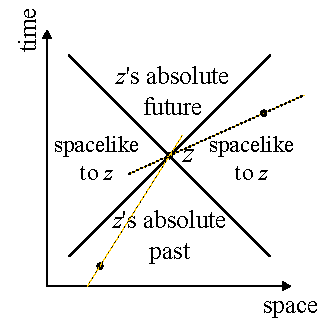
\includegraphics[width=6cm]{relativity-diagram.pdf}
\caption{Points spacelike to $z$, as well as $z$'s absolute past and absolute future. The 
points timelike to $z$ are all of the absolute past and future plus $z$ itself.}
\end{figure}
In some of our arguments, we will give two-dimensional diagrams, where space is the horizontal axis and time
is the vertical axis, and the units are chosen so that the speed of light is equal to $1$. In these diagrams,
an object moving at the speed of light is represented by a line at $45$ degrees to horizontal, while 
lines that are more or less than $45$ degrees to horizontal respectively represent movement at less or more
than the speed of light. (See Figure~\ref{fig:relativity-diagram}.)

\begin{figure}\label{fig:simultaneity}
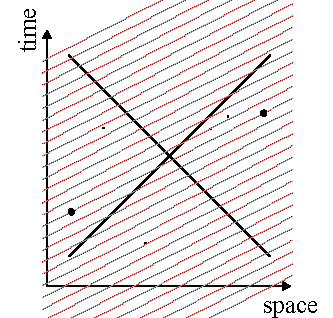
\includegraphics[width=6cm]{simultaneity.pdf}
\caption{A reference frame defined by a collection of parallel hyperplanes. The two black points are simultaneous
according to this frame.}
\end{figure}
Given a reference frame $F$, for any point $z$ in spacetime there will be a set of points in spacetime simultaneous 
with $z$ according to $F$. These points all lie on the same ``hyperplane'' (i.e., a flat three-dimensional slice 
through spacetime). Moreover, these points are all spacelike-related to each other, so we say that this is a 
spacelike hyperplane. A reference frame $F$ then divides up spacetime into a family $S_F$ of parallel spacelike 
``hyperplanes of simultaneity'' such that two points of spacetime are simultaneous according to $F$ provided that they lie on the 
same hyperplane $K$ in $S_F$. In a two-dimensional diagram, the reference frame will be a set of parallel lines
whose slope to the horizontal is less than $45$ degrees. (See Figure~\ref{fig:simultaneity}.)

Conversely, given any one spacelike hyperplane, we can form the set $S$ of all the hyperplanes parallel to it, and this 
set then defines a reference frame $F$ such that $S_F=S$.

\subsection{Of snakes, rattles, form and matter}
\begin{figure}\label{fig:snake}
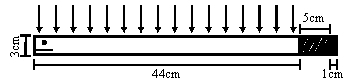
\includegraphics[width=10cm]{snake.pdf}
\caption{An idealized cylindrical snake subject to blasters (arrows). Striped area: non-tip rattle; black area: rattle tip.} 
\end{figure}
Imagine a rattlesnake stretched out in a line from head to tail, with the snake staying still in a reference frame $F$. For concreteness and 
simplicity, let's model the rattlesnake as half a meter long, including a six centimeter rattle, with a thickness of at 
most three centimeters throughout its body. Now something terrible will happen to the rattlesnake. Science-fictional blasters 
are pointed at every centimeter of the  snake's body other than the rattle. These blasters are all timed to have their blasts 
hit the snake simultaneously, in frame $F$, at $t_1$. Once the blast hits the snake, it very quickly vaporizes the section 
of the snake's body it is pointed at. Stipulate that a ``jiffy'' is the very short amount of time it takes light to travel one 
centimeter, about 33 picoseconds,\footnote{This definition is attributed on the Internet to the chemist Gilbert N. Lewis, but 
I have not been able to track 
down an original citation.} and let us suppose it takes four jiffies to vaporize each section of the snake (the section 
is three centimeters thick, so the blast can go from one side to the other of the snake in less than four jiffies without exceeding the 
speed of light). If $t_2$ is four jiffies after $t_1$, then at $t_2$ all that will be left of the snake is the rattle. 

But according to Relativity, causal effects propagate at speeds not exceeding that of light. Now, consider the \textit{tip}
of the rattle, which I will stipulate to be the very last centimeter. At $t_1$, the nearest blast is five centimeters away from 
the tip of the rattle. Since the blasts are the cause of death, and causation propagates at a speed not exceeding that of light,
over the four jiffies between $t_1$ and $t_2$, the effect of the blasts will not yet reach the rattle's tip. 

Now, on an Aristotelian metaphysics, for the rattle's tip to cease to be a part of the snake, the tip
must lose its snake form. This requires that the tip must be affected in some way by the blast. At
$t_2$, however, the tip has yet to be affected, given the speed of light limit.
But as long as the snake form is found in \textit{some} matter, the snake still exists. So 
at $t_2$, the snake exists, even though everything outside the rattle has been destroyed (and presumably the vaporization of 
the section of the snake just next to the rattle has resulted in some of the rattle getting destroyed, too). Thus, as I advertised 
in the previous section, we have seen that the snake can survive as just a part of a rattle.

Likely, this survival is very short: we can reasonably speculate that the loss of snake form proceeds through the rattle 
very fast, maybe even at the speed of light. A few more jiffies, then, and the snake will likely be gone.

One might object that loss of form is not the kind of effect that we have in mind when we say that causal influences do not 
exceed the speed of light. There are two supplementary arguments I can offer here. First, if the tip of the snake's rattle 
has indeed lost its snake form at $t_2$, let $z$ be a spacetime point within the tip of the snake's (no longer alive) rattle 
at $t_2$. Let $E$ be the event of the blasters beginning to blast. Then $z$ and $E$ are spacelike-related, because the spatial 
distance between $z$ and the nearest part of $E$ is five centimeters, while the temporal distance between $z$ and $E$ is four
jiffies, so one cannot travel between $z$ and $E$ without exceeding the speed of light. But if they are spacelike-related, then
there will be a reference frame $F'$ according to which $z$ is earlier than $E$. Thus, in reference frame $F'$, the tip of the 
rattle will have lost its form \textit{before} the blasters went off. This seems very strange indeed.

Second, it is a standard Aristotelian point that a body part that loses its form stops existing. A severed finger is a 
finger in name only: the finger has perished and there is just a heap of matter. Thus, loss of form is the destruction 
of the rattle's tip. But the idea that the blasters somehow managed to destroy the rattle's tip in a faster-than-light 
way is rather implausible. Destruction of objects seems like the kind of thing that shouldn't proceed in a faster-than-light
kind of way, especially since the argument of the previous paragraph shows that the destruction in some reference frames 
would have to preceed the blast. 

As already noted, if a snake can survive---even if only for a few jiffies---as only a rattle, there should be no deep 
difficulty in a human surviving as a cerebrum. 

One might object that rattles are not living and informed parts of a snake, but dead stuff. If so, then replace the 
rattlesnake with a non-rattlesnake in the argument, point blasters at all but the last six centimeters of tail, and 
use the same argument to conclude that the snake can survive as just a few centimeters of tail. This is not quite as 
amazing as surviving as part of a rattle, but it is sufficient to make the \textit{a fortiori} argument above about the 
possibility of survival as a cerebrum.

Finally, note that this snake thought experiment already points our attention towards SET, by showing that it is 
at least \textit{possible} for a large organism to shrink to an insignificant portion at the time of death.  

\subsection{A geometric argument for SET}
First, imagine you are holding a perfect cube. Now imagine putting a perfectly flat plane against the cube. If the 
plane is parallel to and touching one of the six faces of the cube, it will make contact with the whole of the face, 
and hence with infinitely many points. Similarly, if the plane is parallel to and touching one of the twelve edges 
of the cube, it will make contact with the whole of the edge, again with infinitely many points of contact. But in 
every other orientation of the plane against the cube, the plane will contact the cube at exactly one point, indeed at 
one of the eight vertices of the cube. 

Moreover, there is a sense in which there are vastly more orientations of the plane relative to the cube where the 
plane contacts the cube at one point than where the plane contacts the cube at more than one point. There are only 
six orientations where the plane contacts the cube at a face---the plane has to be parallel to taht face. There are, 
admittedly, infinitely many orientations where the plane contacts the cube along an edge, but these orientations 
are constrained by the need for the plane to be parallel to the edge. Once we decide which of the twelve edges of 
the cube to align our plane with, we have only one degree of freedom with regard to the orientation between the cube 
and the plane. Imagine rocking the plane against the cube, keeping contact with the edge---there is only one degree 
of freedom to the rocking. But when the plane makes contact with one of the eight vertices of the cube, there are two 
degrees of freedom—we can rock the plane along two different angles and keep the contact. This geometric observation 
remains correct regardless of what solid object we use in place of the cube. If we place a plane against the boundary 
of the object, for ``almost all orientations'' of the plane, the plane will be contacting the object only at a single 
point. (In the case of some shapes like an ellipsoid, this will be true for all orientations.) Moreover, the same thing is 
true in $n$ dimensions for any $n>1$: if we have an $n$-dimensional object and have an $(n-1)$-dimensional hyperplane rest 
against it, for almost all orientations of the hyperplane, the object will contact the hyperplane at a single point. 
(This is made mathematically precise in the Appendix.)

\begin{figure}\label{fig:geometric}
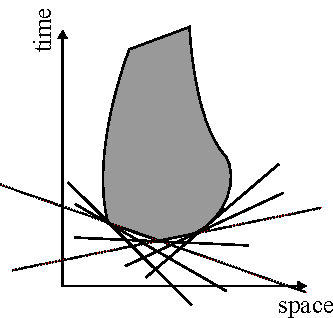
\includegraphics[width=6cm]{geometric.pdf}
\caption{Only two hyperplanes with slope less than $45^\circ$ meet the beginning boundary of the gray object in more than one point.}
\end{figure}
Now move to the four-dimensional spacetime of Special Relativity and consider a material substance with a beginning and end to 
its life, say Rover. Let $D$ be the four-dimensional shape consisting of the points of spacetime occupied by Rover, and 
imagine a reference frame $F$. This reference frame has a simultaneity relation defined by a family $S_F$ of spacelike 
hyperplanes, where, recall, two points are simultaneous provided that they lie on the same hyperplane in $S_F$. Assume $D$ is 
finite in size, both spatially and temporally (i.e., no more than $x$ meters in diameter at all times and no more than $y$ seconds in temporal 
extent, for some finite $x$ and $y$). Suppose $z$ is one of the points of 
spacetime where Rover begins to exist with respect to frame $F$. Let $K$ be the hyperplane in $S_F$ that passes through 
$z$. This will be a hyperplane resting against $D$. If Rover begins to exist at two or more points according to frame $F$, 
then $K$ will make contact with two or more points of the boundary of $D$. Now, for almost all 
orientations, a hyperplane of that orientation that rests against the object will make contact with the object's boundary 
at a single point, as discussed earlier. Moreover, the orientation of a spacelike hyperplane defines a reference frame (since the
orientation of a hyperplane is sufficient to determine the family of parallel hyperplanes). Thus, according to almost all 
reference frames, Rover begins to exist at a single point. (See Figure~\ref{fig:geometric} for a two-dimensional
illustration.)
Exactly the same argument applies to Rover's demise: at almost all reference frames, Rover ends its life at a single point.

A few words are needed about what is meant by ``almost all'' reference frames. A reference frame is defined by the 
orientation of its hyperplanes. We can define an orientation of a hyperplane $K$ by a four-dimensional vector $v$ that is 
perpendicular to $K$ and has length one. The set of all such vectors is a hypersphere of radius one (the set of points in 
four-dimensional space of distance one from the center), though we are not interested in the whole hypersphere, but only in 
the part of it that corresponds to vectors that are perpendicular to spacelike hyperplanes.\footnote{$^*$It is important for 
technical reasons that this part has non-zero hyperarea.} Now let $U$ be the set of all the unit-length vectors $v$ such that 
(a)~the vector $v$ defines a reference frame (by defining a family of spacelike hyperplanes perpendicular to $v$) and (b)~in 
this reference frame Rover starts existing at two or more points. Then $U$ has zero hyperarea as a portion of the hypersphere 
of all vectors of radius one. Mathematicians refer to something that happens in a region of zero area, volume, or similar 
measure as happening ``in almost no cases'', and to what happens everywhere outside such a region as happening ``in almost 
all cases''. It follows that in almost reference frames, Rover starts existing at only one point, and ends at only one.  
A more precise version of this argument will be given in the Appendix.

Our argument assumed that Rover has finite extent in both space and time. Suppose now Rover has infinite extent in time but 
is still bounded in space---i.e., at all times, Rover is contained in some ball of finite diameter.
There are three possibilities: (i)~Rover has neither beginning nor end, (ii)~Rover has a beginning but no end and (iii)~Rover
has an end but no beginning. 

Regarding (i), Rover is irrelevant to SET because SET claims that all the beginnings and endings of 
material substances are subatomic, and if Rover lacks a beginning or end, then Rover does not contribute to the collection of 
beginnings and endings of material substances. 

Case (ii), where Rover has a beginning but no end, requires a minor tweak to the argument. Just apply the above argument to 
a finite-duration initial temporal part $R_1$ of Rover of sufficient temporal duration (as measured in whatever frame 
you like)
so that in all reference frames Rover's beginning occurs within $R_1$. And case (iii) is very similar: just apply the argument to 
a sufficiently long but finite-duration final temporal part $R_2$ of Rover.

What remains is the case of material substances that have infinite spatial extent. Here I suggest a simple hypothesis: there aren't
any such. The only at all plausible candidate for such a thing would be the universe as a whole, and given the Aristotelian 
thesis that substances can't have substances as proper parts, and the fact that we are substances and would be part of the universe,
we have to conclude that there is no such substance as the universe. If I am wrong about that, then as far as my arguments go,
I will need to restrict SET and SBT to substances other than the universe, which does not affect any of the applications I will
make.

Thus, if we fix a random reference frame, we can be all but certain that any specified material object has a point-like 
beginning with respect to the frame if it has a beginning at all, and it has a point-like ending if it has an ending. In fact, 
as long as the number of material objects in 
the universe with finite lifetime is finite or countably infinite, then for any fixed random reference frame, we can be all 
but certain that \textit{all} of them start off and end up subatomic in size. (This follows from the mathematical fact that the 
union of a countable collection of sets of measure zero has measure zero.) When I initially gave the Small Endpoints Thesis, 
I didn't specify a reference frame. The above argument is compatible with the existence of some reference frames where SET is 
false. However, the argument shows that for any fixed frame the reader might have in mind---say, a frame defined by some 
precisification of the reader's current center of mass---it is nearly certain that SET is true in that frame, since 
almost all frames have SET true in them. It would require incredible luck for the reader to have in mind a reference 
frame where SET is false—luck akin to tossing a coin infinitely many times and getting heads each time. I assume the reader is not so lucky.

\subsection{A causal argument}
An object exists as soon as any part of it exists. Moreover, absent backwards causation, whether an object 
exists at a time $t$ never depends on what happens after $t$. This thesis when combined with some additional 
considerations about causality and Special Relativity yields an argument for the Small Beginnings Thesis, 
that material objects with finite lifetimes start off subatomic. 

Now, for a reductio, suppose that Rover is a material object whose life occupies a bounded region of 
spacetime and that Rover does not start off subatomically small in some reference frame $F_1$. For simplicity, 
I will assume that Rover has a first moment, $T$, of existence with respect to $F$. This is not guaranteed. 
It could be that Rover exists at all moments t after some time $T$ but not at $T$ itself. The argument could 
generalize to that case, but becomes more technically complicated.

\begin{figure}\label{fig:causal}
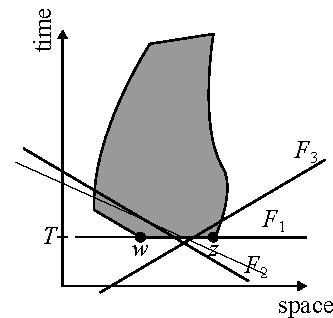
\includegraphics[width=6cm]{causal.pdf}
\caption{In $F_1$, $w$ and $z$ are simultaneous, but in $F_2$, $w$ comes first, and $F_3$, $z$ comes first.}
\end{figure}
All material objects have causes. Let Spot be Rover's cause. Then Spot in causing Rover acts on Rover at at 
least one spatiotemporal point, $z$, which point is at a time $T$ and within the boundary of Rover's four-dimensional
region. Since we have assumed Rover is not subatomically small, there is another spatiotemporal point at time $T$ 
and within Rover, which point we will call $w$. Because $z$ and $w$ are simultaneous with respect to frame $F_1$, 
they are space-like related, and it follows that there is another reference frame, $F_2$, according to which $w$ is 
earlier than $z$ (see Figure~\ref{fig:causal}).

Now, let's think about how things look in our new frame $F_2$. Since Rover exists at $w$, and $w$ is earlier than $z$, what 
happens to Rover at $z$ is causally irrelevant to Rover's existence. Hence Spot's causal activity at $z$ is causally 
irrelevant to Rover's existence. But causation should be something that does not depend on reference frame. This 
thesis is intrinsically plausible and is also implicit in standard ways to think about Relativity 
Theory.\footnote{For instance, one of the reasons why faster-than-light causation is problematic is 
that if event $C$ caused event $E$ in a faster-than-light way in one reference frame, then in another reference 
frame event $E$ would be prior to $C$, and so the causation from $C$ to $E$ would have to go backwards in 
time. But this argument against faster-than-light causation only works if causation is not dependent on the reference 
frame. If causation were dependent on a reference frame, we could simply say that in the second frame, event $C$ 
does not cause $E$.}  So we have a contradiction: Spot's causal activity at $z$ both is relevant and not relevant 
to Rover's existence.
 
It is worth noting that there is a further detail to the beginnings of material substances that we do not get on the 
geometric argument but follows from an extension of the causal argument. The geometric argument is compatible with a material substance 
beginning at different spacetime locations in different reference frames. Imagine that the material substance is smoothly 
rounded at its temporal beginning. Then different spacelike supporting hyperplanes on the ``bottom'' (i.e., temporally earlier) 
side of the four-dimensional region occupied by the substance will contact the hyperplane at different points. (Imagine supporting hyperplanes for 
a four-dimensional ball: they all meet the ball at different points.) Each such hyperplane defines a different reference frame,
and in each reference frame then the object will begin at a different point of spacetime (namely the contact point between 
the hyperplane and the boundary of region occupied by the substance). 

But an extension of the causal argument does not allow this. For suppose that that in frame $F_1$ Rover begins at 
point $z$ in spacetime and in frame $F_2$ Rover begins at a different point $w$ of spacetime. If $z$ and $w$ are spacelike 
related, then there will be a third frame $F_3$ where $z$ is earlier than $w$ (see Figure~\ref{fig:causal}). Then, much as in the orginal argument, 
relative to 
$F_3$, Spot's causal activity at $w$ comes after Rover has already come into existence at $z$, and hence is irrelevant to 
Rover's 
existence, a contradiction. Suppose now that $z$ and $w$ are not spacelike related. Then one of them will be \textit{absolutely}
earlier than the other. Swapping labels if necessary, we can suppose that $z$ is the earlier one. But then Spot's causal
activity at $w$ will come after Rover has come into existence relative to \textit{all} frames, and hence will be
irrelevant.

Assuming causal influences travel at the speed of light, this argument also yields a picture of what the temporal beginnings of 
a material substance are like. They are sharp and pointy. For if the substance absolutely starts at point $z$ due to Spot's 
causal activity, and causal influences travel at the speed of light or less, then all of the region occupied by Rover needs
to be contained in the region reachable from $z$ at the speed of light or less, i.e., in the future light-cone with vertex $z$.
Thus Rover has a sharp point at its beginning.\footnote{Or at least sharp in the natural units of physics where the speed of 
light $c$ is $1$. In such a unit system, lightcones subtend a $90$ degree angle at their vertex. In a unit system where the 
speed of light is a large number, light cones are much blunter.}

\subsection{Subatomicity}
I advertised the endpoint claims as holding that beginnings and endings are subatomic, but the actual relativistic 
arguments seem to prove something stronger: that the beginnings and ends are points.

There are, however, several reasons for preferring the weaker ``subatomic'' formulation. First, the arguments are based
on Special Relativity, and assume a spacetime continuum. It might, however, turn out that this is only an approximation 
to an underlying discrete spacetime. Assuming that Special Relativity is a sufficiently good approximation, our arguments may 
still work approximately, but break down at a sufficiently small scale. That scale is very likely to be something like the 
Planck length scale, which is very much subatomic. So maybe all we get are subatomic endpoints.

Second, on interpretations of Quantum Mechanics other than Bohmian ones, particles do not have precise positions. The arguments 
appears to point towards substances beginning as single fundamental (and hence subatomic) particles, but the positions of these
particles may be fuzzy and not pointlike. 

Third, our arguments are compatible with a scenario on which material substances only approach pointlikeness asymptotically
as we approach their beginnings and ends. The first argument, in the more precise formulation it has in the 
Appendix, yields the claim that in almost all reference frames, the hyperplane marking the beginning or the end of the 
substance intersects the boundary of the spacetime region occupied by the substance at a single point. However, the boundary
of the spacetime region occupied by the substance need not itself be occupied by the substance. The substance might only 
occupy the \textit{interior} of the region, not including the boundary. In such a case, the endpoint hyperplane does not actually
intersect the region occupied by the substance, and the region of nearby hyperplanes occupied by the substance will asymptotically
tend to a point.??forwardref  A similar remark can be made about the second argument if we drop the simplifying assumption that
the substance has a first moment of existence.

\subsection{Applications of SET/SBT}
\subsubsection{Cerebra and zygotes}
An immediate consequence of SET/SBT is that there is no special metaphysical difficulty in an animal's 
surviving as a cerebrum. After all, a cerebrum is many orders of magnitude more organized than a subatomically-sized
substance. Similarly, those who think that we could not have been zygotes because zygotes are insufficiently sophisticated
to support our existence must abandon this argument given that we---and all other material substances with beginnings---started
off even less organized than a zygote, namely subatomic. Of course, the relativistic considerations above do not 
show that we were once zygotes or that we would in fact go with a cerebrum in a cerebrum transplant. As far as the relativistic 
considerations go, we might have started our lives as subatomic objects within the pinkie of a biologically two-year-old 
body, and we might end our lives as subatomic objects in a big toe (compare the rattlesnake argument, after all, in ??backref).
But it seems more in keeping with the anti-skeptical bent of Aristotelian optimism to think that we start and end our lives 
in a somewhat less counterintuitive way.

\subsubsection{Proper disposition of matter}\label{sec:disposition}
It has been commonly believed by Aristotelians that in order to receive a form, matter must be properly disposed??ref, and,
conversely, form departs from matter precisely when the disposition of matter becomes inadequate. However, given that a subatomic chunk of living human matter cannot be distinguished from a subatomic chunk of living oak tree matter or a subatomic chunk of a dead cat, the disposition thesis becomes insupportable as it stands. 

Nonetheless, one might be able to defend a version of the disposition thesis where one considers the ``adequate disposition'' of 
a piece of matter to be in part a function of the environment the matter finds itself in. Thus, one might hold that a subatomic
pointlike piece of matter whose environment is the rest of a just-fertilized or about-to-be-fertilized zygote counts as 
properly disposed to receive the form, and a subatomic pointlike piece of cerebral matter whose environment is a cerebrum that 
has lost or is about to lose its functioning counts as no longer properly disposed to hold on to the form. Such proper
disposition facts could be grounded in the causal powers of the parents, in the case of the beginning of life, or in the causal 
powers of the substance to ``give up the ghost and create a corpse'', in the end of life cases. 

There is independent reason to think that the adequate disposition thesis depends on relational features of the matter in 
question. Start with an artifactual example. Michelangelo is said to have remarked that his statue was already there in the 
marble but needed to be freed.??ref It seems more in keeping with common sense ontology, however, to say that the statue came 
to exist only once enough of the outside marble was chipped away. In other words, the existence of the statue required the 
matter of the statue to have an adequate environment: one lacking marble all around. While statues may not actually be substances,
we can imagine biological examples. Suppose, for instance, that suddenly new matter appeared in all the empty spaces between the particles of our body, thereby blocking all functional behavior. Of course, we would soon suffocate and die, but it is plausible
that even before that it would be correct to say that the body is no longer adequate to its function. The empty spaces
in our bodies are crucial to our functioning, and so a part of the material adequacy of the human body for its human form 
is having such empty spaces, which is an environment-relative feature.

That said, while it is plausible that the causal structure of our universe is such as to tie our life to matter in an
appropriate environment, once we see that a defensible proper disposition thesis must involve relational features of our matter, it 
becomes intuitively less plausible to suppose that the proper disposition thesis is \textit{metaphysically} necessary. We may have 
the causal power to ``give up the ghost and create a corpse'' under certain inadequate conditions, but 
our finite causal powers could be overridden by other powers, and hence it would be metaphysically possible for us to continue to 
exist in such cases. Indeed, it seems central to the concept of a material substance that it enjoys an \textit{ontological} independence of material stuff outside of itself. 

It was essential to the normative applications of Aristotelian forms??backref, and the philosophy of science
considerations??backref, that we understand
the forms in a robust way, and not as merely ontologically grounded in the arrangement of matter. The relativistic arguments provide a powerful metaphysical consideration in favor of such a robust account of form. For if substances begin their existence
at a subatomic level at which one cannot distinguish the substance's matter as constituting a living human or a piece of organic
slime, then form cannot be grounded in the arrangement of the matter that it is the form of. 

It is worth noting that the Small Endpoints Thesis argument against the adequate disposition thesis is still compatible with 
a weaker version on which there are \textit{some} appropriateness conditions on the matter that can have a given form. Perhaps there 
are few if any restrictions on the \textit{arrangement} of the matter, but we can have restrictions on the \textit{type} of 
matter. Perhaps, say, humans and oak trees must be made of the fundamental particles of the Standard Model of physics,
because it could be that human and oak forms require particles tied to the kinds of laws of nature that our world has.
Perhaps even more restrictively, the bodies of earth animals must be made of matter rather than antimatter. Such restrictions
are possible, but do not appear to have significant philosophical applications.

The Small Endpoints Thesis rules out significant positive adequacy conditions on which a body must have some significant and 
distinctive structure to receive a form. However, it is compatible with the thesis that are significant \textit{negative} adequacy 
conditions. Thus, while a pig and a sparrow might start as a very similar subatomic entity, one might hold that a \textit{developed}
pig-like body could not have a sparrow form and a \textit{developed} sparrow-like body could not have a pig form. For instance, 
one might hold that having DNA is not a necessary condition for being either a pig or a sparrow (since the subatomic entity 
does not have DNA), but having sparrow DNA is incompatible with being a pig and having pig DNA is incompatible with being 
a sparrow. But while such a thesis is coherent, it does not appear to be well-motivated metaphysically. A sparrow embryo and 
a pig embryo appear to have more similarity to each other than either of them has to a subatomic entity. If both the sparrow 
embryo and some subatomic entity can have the same form, why would it be metaphysically impossible for the pig embryo to have 
it? 

In response, one might hold that a pig form only has the power to inform matter that falls somewhere along the line of 
development from a subatomic entity to the matter of a zygote with pig DNA to the matter of a recognizable embryonic pig to 
the matter of a recognizable mature pig. But why think it has such a restricted power of informing? It does not seem any 
``metaphysically harder'' for the pig form to inform a sparrow-like body than to inform a subatomic entity. We should not 
posit metaphysical restrictions without positive reason.

\subsubsection{The special composition question}
Finally, observe that the arguments for SET and SBT are independent of Aristotelian hylomorphism (though the 
causal argument presupposes a realism about causation). Therefore, they can be used
to criticize a number of alternative answers to the special composition question---the question of giving informative 
necessary and sufficient conditions for a plurality of entities to compose a whole.\footnote{??Ref}  
Recall that the two extreme answers are nihilism, which holds that a plurality of two or more objects never 
composes a whole, and universalism, which holds that every plurality of objects composes a whole. All other answers are  restricted theories of composition, including the Aristotelian answer defended in 
??backref.

Now, SBT gives us good reason to think that for any material substance, say a cat, there is a time when 
that substance is complex and yet roughly the size of a small molecule (say, H$_2$O). For the substance starts subatomic, 
and it is implausible that it would suddenly jump over all the intermediate sizes and be the size of a small molecule.
We expect growth to be fairly continuous. This means that the correct answer to the special composition question
has to be such as to be applicable to things the size of a small molecule. Van Inwagen's answer??ref that the $x$s compose
a whole just in case they have a life together (understood in the usual empirical biological way, rather than in terms of having 
a form of a living thing) fails this condition---things that small do not have a life together. We can expect other 
accounts based on macroscopic relations or properties to fail. Thus, it fits with many of our intuitions that the $x$s 
compose a whole just in case they either have a life together or someone has a purpose for their joint function, since
that allows not just living things but also artifacts into our ontology. But according to SBT plus a continuity constraint,
if a chair is actually a substance, at some point that substance is localized as a very, very tiny complex substance.
But while a carpenter has a purpose for the joint function of the parts of a chair, the carpenter has no purpose for any 
such mysteriously tiny substance at the root of the chair. 

Mereological universalism is usually elaborated as a four-dimensionalist view: any plurality of object-stages across 
spacetime composes a whole. Such a four-dimensionalist mereological universalism massively violates SBT: there will be 
many material objects with large beginnings. 

On the other hand, an Aristotelian account with a metaphysically robust view of form has no special difficulty with 
tiny things. An oak tree may at some point consist of a single atom, but it can simply be an empirically inaccessible 
fact that that atom has an oaken form. 

\section{Persistence and death}
\subsection{Causal powers}
Living substances appear to causally contribute to their future existence---dogs that eat healthy food and trees that succeed
in processing sunlight are apt to live longer. Let's take this appearance at face value. This suggests that living substances
have a causal power to continue existing given an appropriate environment. The same is likely to be true of non-living material
substances as well. 

This is a generalization about the causal powers of things, rather than a general principle of ``existential inertia''.??refs
And as in the case of other causal powers, we can expect there be activation conditions for the power of self-continuation.
Our relativistic arguments give us reason to think these activation conditions include not just the intrinsic features 
of the substance, but features of its immediate environment as well. When these conditions are not met, a living 
substance instead of continuing its bodily existence excretes its matter, thereby generating a corpse. 

If the Small Endpoints Thesis is correct, the generation of a corpse is not an instantaneous process. At the end of its 
life, a horse is subatomic. But empirically it is obvious that, in typical horse deaths, throughout the death process there 
is matter arranged in the shape and size of a horse. Thus, when the horse is subatomic, most of its corpse has already been
generated: the horse at the end of its life has shrunk to a subatomic substance within a nearly fully formed corpse. We might speculate
that once the internal and environmental conditions for the horse to cause its future existence start failing, the form's 
activity contracts its scope, generating a corpse where the form is no longer informing the body. Towards the end
of the process, only a subatomic portion of the body is informed by the form. It is plausible that the transition from 
the form informing hundreds of kilograms of horseflesh to its informing a subatomic portion is continuous, though it may be 
very fast, and thus we have a continuous process of corpse-generation. 

It may seem initially strange to think that a living organism coexists with corpse-matter. But in a way we always do 
that. Bits of us are constantly dying: our skin is literally turning to dust. That dust flies way from us. It's just
that at final death the process becomes more complete---what looks like our body is eventually mostly a heap of dead matter, and then finally wholly so. 

\subsection{The possibility question}
Is it metaphysically possible for the human form survive the destruction of the human body? If we think of the form in a non-robust way as 
a shape or arrangement of matter, then a form without matter is as 
impossible as the smile without the Cheshire cat. However, form on the account defended in this book is highly robust. 
As we saw in ??backref, it grounds normative and nomic facts. And as our relativistic arguments show, the form cannot
be ontologically grounded in the arrangement of matter, since material substances begin their existence at such a tiny---indeed, subatomic---scale  that we should not expect any intrinsic difference between the initial matter of a human, a cat or a mushroom.

At the same time, while we have good reason to think that a substance's form does not ontologically depend on the specific type or arrangement of matter, it could be that the form requires some matter or other for its existence. But while there is some intuitive 
reason to think that the human form should be tied to a specifically human body and the oaken form to a specifically oaky body,
once we have rejected this intuition, it is not clear that there is a significant reason to think that the form 
metaphysically requires any 
matter for its existence. 

One might think that without a body to inform, a form has ``nothing to do''. Aquinas famously responded to this line of thought
by saying that the human form was a soul with an abstract intellectual function that did not depend on a body.??ref This response may 
be correct, but we need not settle the point right now. For even if something has ``nothing to do'', it does not follow that 
it has to cease to exist. The question we are examining in this section is one of possility: \textit{can} the human form survive the 
destruction of the body. If the form no longer had anything to do after death, Ockham's razor would give us reason to think that the form would cease to exist. But Ockham's razor is a principle about what \textit{actually} exists, not what \textit{possibly}
exists. We should not suppose actual conspiracies when there is a simple explanation, but we should all agree that conspiracies
are \textit{possible}. 

That said, a form without a body could still have a metaphysical ``task'': it could ground the \textit{possibility} of matter coming back
to re-form the old substance. 

Given the robust nature of form, and its ontological independence of the details of the arrangement of matter, we have some 
reason to think that it is metaphysically possible for form to survive the destruction of the body, not just in the case of 
human form, but of any form of a material substance.

\subsection{The actuality question}
The next question is whether the human form actually survives the death of the body. Aristotelian optimism makes it very 
plausible that beings of a given kind are capable of approximating the flourishing proper to that kind, and indeed that such 
an achievement is not just a rare exception. But human flourishing is rarely if ever even approximated in this life, so we have 
good reason to think that human existence can be expected to continue past death, and not merely in rare exceptional cases. 

For consider both the moral and the intellectual aspects of our flourishing. As Aristotle himself knew??ref, true virtue is 
rare. When we look at ourselves, we see that all too often even actions that are right do not flow from motives far from 
right, and in this we are not exceptions among humans. We may have friends, but we do not cherish them nearly as we ought. 
Every human around us is something with dignity, something sacred (we need not understand this in a religious sense), a being capable of morality, love and knowledge. We should be constantly in awe of our fellow humans and constantly grateful for being allowed 
to partake of the community of such beings. And yet we are usually far from that awe---often we even look down on others. 

On the intellectual side, we know how quickly a child's questions can lead far beyond human knowledge. The physicist 
Richard Feynman wondered as a child why it is that a ball in a wagon would move back in the wagon when the wagon was 
pulled. His father explained that objects have a tendency to stay put or continue moving (``inertia'') but then correctly
emphasized to little Feynman that we have no idea why they do that.??ref Our scientific questions bottom out with laws of nature,
but few if any of us know what makes them hold: there are many views on the grounds of laws of nature; even if one among these is 
true, it is likely that only few believe that view, and even fewer---if any---know it to be true. Yet any child or any adult 
either wants to know or \textit{ought to} want to know. We learn the answers to non-ultimate questions of detail, but what is 
really important to our intellectual flourishing are the ultimate questions. For our intellectual flourishing calls for a holistic
understanding of reality. And yet we are so far from that.

Given our vast distance from flourishing in this life, Aristotelian optimism indeed supports the actuality of a life
after death.

\section{Naturalism}
Is the Aristotelian hylomorphic account of humans compatible with naturalism? This depends on how naturalism
is defined and whether we take the theistic version of the account or not.

Since theism implies the existence of a non-natural causally efficacious substance, namely God, it will be incompatible
with most versions of naturalism. In Chapter??ref I will argue that the best version of the Aristotelian account
will be theistic.

Bracketing theism, it is interesting to query whether the Aristotelian's account of the forms of finite
substances is compatible with naturalism. If so, then one could at least combine the Aristotelian account with 
naturalism at least for finite objects like us, and save some naturalistic intuitions. Furthermore, it would mean
that an Aristotelian not convined by the arguments that theism is needed to make the theory satisfactory could
be a full-blown naturalist.

If we take naturalism to say that the only entities that exist are the ones that would figure in a completed science,
then it is unlikely that Aristotelian metaphysics would be compatible with naturalism about finite objects. However,
such a strong naturalism would likely also conflict with many other metaphysical theories that are rarely taken to 
contradict naturalism. 

For instance, consider theories of time. Of the theories of time, four dimensionalism, on which
ordinary objects like ourselves are extended in time as well as space, is what seems to fit best with Relativity Theory. 
But the most common four-dimensionalist view of changing properties is perdurantism: changing objects are made of temporal parts or
slices to which the properties are primarily attributed, so that a tomato that once was green and now is red has a green temporal part
and a red temporal part. But slices are unlikely to figure in a completed science if
our current science is a good guide to that. Consider that our current physics considers particles
like electrons and quarks to be fundamental, and hence not made up of smaller parts. But electrons and quarks change over
time (e.g., with respect to spin and flavor), and so they would need to have temporal parts.  But these parts are not found
in our physics: our physics does not go more fundamental than the fundamental particles.

Or consider that our science may quantify over physical objects like particles and fields, and applies predicates to them, but 
does not quantify over properties. Thus, properties, whether understood as universals or as tropes, go beyond current science.
Yet it seems implausible to understand naturalism as implying nominalism.

One may weaken naturalism to say that the only \textit{causally relevant} entities are those of a completed science. But 
this would still rule out perdurantism, since objects change with respect to causally relevant properties, and hence their
temporal parts have these properties, and have them more fundamentally. It would also likely rule out many versions of trope
theory, since the causal efficacy of tropes is supposed to explain the causal efficacy of the objects made of them.

Let's step back. Naturalism denies the existence of causally efficacious ``supernatural'' entities like 
ghosts, but it is neutral on temporal parts and tropes of ``natural'' entities like electrons. 
What is the relevant difference between ghosts and temporal parts of electrons? It seems to be this. While
neither entity is posited by science, if ghosts exist, then certain phenomena that it belongs to science 
to investigate have no scientific explanation, barring systematic overdetermination. If there are ghosts,
they are presumably responsible for at least some of the appearances of ghosts, such as maybe chills some 
people feel in graveyards. These phenomena then either have no physical explanation at all, or by a massive
coincidence are overdetermined by a physical and a spectral cause. There is a competition, thus, between 
scientific and spiritual explanations when we are concerned with ghosts. 

On the other hand, there is no overdetermination in the case of the objects studied by science and their ontological
constituents such as temporal parts or tropes. When a temporal part or a trope of an ice cube makes 
your hand cold, the ice cube also makes your hand cold. The ice cube's cooling causal influence on your hand
does not compete with the ice cube's temporal part's causal influence on you or on the causal influence of 
a trope of coldness (if there are temporal parts of ice cubes or tropes of coldness). Nor is this overdetermination,
since it is not overdetermination when an object $C$ causes an effect $E$ by means of $C$'s part. After all,
it is not overdetermination when you have an ice cube on your hand, and \textit{both} the ice cube and its lower half
cool the hand.

We might thus want to say that naturalism holds that any phenomenon that it falls within the purview of science 
to seek for causal explanations of either has no causal explanation at all, or else has a scientific causal explanation 
and is not overdetermined by a scientific and a non-scientific one. On this account, theism is incompatible with
naturalism if there is a first state of physical reality. For if there is such a state, it belongs
to science to seek for its causal explanation. However, there is a theistic explanation of that state and no 
scientific explanation. We thus have the kind of competition that naturalism rules out.\footnote{If there is 
no initial physical state, we can apply the above argument to an initial
segment of physical states.} One might object that science knows that it cannot, on pain
of vicious circularity, provide a scientific explanation of the first physical state, and hence it does not belong to
science to seek that explanation. But this objection confuses the first physical state \textit{qua} first and the
first physical state as it intrinsically is. It does not belong to science to seek the explanation of the first physical
state \textit{qua} first. But if we just consider it as a specific physical state---particles and fields arranged thus-and-so---then
it certainly belongs to science to seek for its explanation, though that search will be rightly abandoned if sufficient evidence
is gathered that the state is in fact the first one.

Now, let's go back to Aristotelianism. Bracketing theism, the main entity that might trouble the naturalist is form.
But the forms of things are components of substances---humans, dogs, oaks, etc.---that are also found in our current
science (e.g., biology) and are likely to be found in the completed version of that science. And there is neither
competition nor overdetermination between causal explanations provided by
forms and their substances. As long as the substances do not have spooky causal powers beyond the scope of science,
adding forms to the ontology no more contradicts a plausibly defined naturalism than perdurantism or trope theory
does.

It is, of course, open to the Aristotelian to suppose that some finite substances, whether natural like humans and oaks 
or  supernatural like angels or ghosts, have causal powers of a sort that goes beyond the scope of science. But nothing in the applications given for Aristotelianism
posits such powers. Thus as far as the argument of this book goes, there is no contradiction with a carefully
specified naturalism with respect to finite things.\footnote{I think the most plausible place to look for a tension 
would be in examining human free will, but that goes beyond the scope of this book.}

\section*{$^*$Appendix: Making the geometric argument for SET more precise}
Consider a non-empty region $D$ of an $n$-dimensional Euclidean space. Technically, Special Relativity happens in a 
Minkowskian space. But we can embed a Minkowskian space into Euclidean space coordinate-by-coordinate, and will do so 
to make things easier to imagine.

A \textit{hyperplane} is an $(n-1)$-dimensional linear substance of $D$. A \textit{supporting hyperplane} for $D$ is a hyperplane $K$ such that (a)~$K$ intersects the  boundary of $D$, and (b)~all the points of $D$ lie on $K$ and/or one side of $K$. Here, the boundary of a region $D$ is understood in the topological sense, as the set of points $z$ such that there are points of $D$ that are arbitrarily close to $z$ and there are points outside $D$ that are arbitrarily close to $z$. To make (b) more precise, note that $K$ cuts space into two halves, $H_1$ and $H_2$, known as “open half-spaces” such that no two of the three sets $K$, $H_1$ and $H_2$ have any points in common. Condition (b) says that $D$ is a subset of $K\cup H_1$ or a subset of $K\cup H_2$.
Note that a supporting plane for $D$ can intersect $D$ only at a boundary point of $D$. 

Given a vector $v$ of length one (a ``unit vector'') and a plane $K$ perpendicular to $v$, one of the half-spaces that $K$ cuts space into lies in the direction of $v$ from $K$ and the other region lies in the direction of $-v$ from $K$.  We then have this 
useful fact which will be proved later.

\begin{lem}\label{lem:one-supp} Let $D$ be a bounded non-empty region of $n$-dimensional Euclidean space, and let $v$ be any vector. There is exactly one supporting plane $K=K(D,v)$ for $D$ such that (a)~$K$ is perpendicular to $v$ and (b)~no point of $D$ is found in the open half-space in the direction of $v$ from $K$.
\end{lem}

(A region is bounded provided there is some finite $r$ such that every point of the region is within distance $r$ of the origin.) Moreover, \textit{every} supporting plane is of the form $K(D,v)$ for some unit vector $v$: just choose $v$ to be one of the two unit vectors perpendicular to $K$, in such a way that $D$ is on the correct side of $K$ with respect to $v$. Now, the set of unit vectors forms the hypersphere $S^{n-1}$. Then we have (and again the proof will be given later):

\begin{prp}\label{prp:support-zero}
Let $D$ be a bounded non-empty region of $n$-dimensional Euclidean space. Let $U$ be the set of points $v$ on the 
$(n-1)$-dimensional unit hypersphere $S^{n-1}$ such that the supporting plane $K(D,v)$ meets the boundary of $D$ at two or more points. Then $U$ has zero $(n-1)$-dimensional Lebesgue measure as a subset of the hypersphere.
\end{prp}

We are now ready to give a more precise version of the Rover argument. Start with:

\begin{prp}\label{prp:distance} Let $D$ be a bounded region of $n$-dimensional Euclidean space, and let $K$ be a bounding hyperplane for $D$. Suppose the boundary of $D$ intersects $K$ in a single point. Then for any distance $r>0$, there is a $u>0$ such that for every hyperplane $L$ parallel to $K$ whose distance from $K$ is at most $u$, the intersection of $L$ with $D$ is contained in some ball of radius $r$.
\end{prp}

Again, the proof will be given later.

Proposition~\ref{prp:distance} tells us that not only is the intersection of Rover's four-dimensional
boundary with a bounding hyperplane small for almost directions of bounding hyperplane, as we learned from 
Proposition~\ref{prp:support-zero}, but for almost all directions, planes parallel to and sufficiently near
a bounding hyperplane of that direction will have an arbitrarily small intersection with Rover. Thus, for almost
all reference frames $F$, if we look at Rover's lower temporal bound or beginning time $t_0$ in $F$, for any fixed
non-zero size $\delta$, at all times $t_1>t_0$ shortly after that lower temporal boundary (i.e., with $t_1-t_0$ 
small), Rover will still have size no bigger than $\delta$.\footnote{To make the point even more precise, we should
consider the conversion factor between three-dimensional spatial size relative to $F$ and the four-dimensional Euclidean distances in Proposition~\ref{prp:distance} on a hyperplane $L$. However, all we need for the argument is that if 
each distance is non-zero so is the other and if one distance tends to zero so does the other.}

Similarly, the points of contact between $K_2$ and $D$ can be characterized as Rover's upper temporal boundary with respect to $F$, and the exact same argument shows that for almost all frames $F$, Rover ends its life smaller in size than any specifiable positive size, and hence it is subatomic.

We can now prove our Lemma and Propositions.

\begin{proof}[Proof of Lemma~\ref{lem:one-supp}]
Let $c$ be the supremum of the dot product $v\cdot x$ as $x$ ranges over $D$. This is finite as $D$ is bounded. Let 
$K$ be the plane $\{ z : v\cdot z = c \}$, which is perpendicular to $v$. Any point $z$ in the open half-space $H$ defined by $K$ in the direction of $v$ satisfies $v\cdot z > c$, and hence is not in $D$. Let $(x_i)$ be a sequence of points of $D$ such that $v\cdot x_i$ converges to $c$. Let $y$ be a limit point of the $x_i$ (this exists since $D$ is bounded). Then $y$ is in the topological closure of $D$. But $v\cdot y = c$ by continuity of the dot product, and there are points arbitrarily close to $y$ in the half-space $H$ and hence not in $D$, so $y$ is in the boundary of $D$. Since all points $z\in D$ satisfy $v\cdot z \le c$ by choice of $c$, it follows that $K$ is a supporting plane for $D$.
 
Now, let $L$ be any supporting plane for $D$ perpendicular to $v$ such that no point of $D$ is found in the open half-space in the direction of $v$ from $L$. Then $v\cdot z$ takes the same value for all $z \in L$, since $L$ is perpendicular to $v$. Let that value be $d$. We then have $v\cdot z \le d$ for all $z\in D$ since no point of $D$ is found in the open half-space in the direction of $v$ from $K$. It follows by choice of $c$ that $c \le d$. Now, since $L$ is a supporting plane, it meets the boundary of $D$, and so there is a sequence $(u_i)$ of points of $D$ converging to a point $w\in L$. Thus, $v\cdot u_i$ converges to $v\cdot w = d$ by  the continuity of the dot product. We have $v\cdot u_i \le c$ for all $i$ by choice of $c$, and so $d = v\cdot w \le c$.
Thus $c = d$, and so $L = K$.
\end{proof}

\begin{proof}[Proof of Proposition~\ref{prp:support-zero}]
A convex set is one that contains the line segment between every pair of points in it. The closed convex hull of $D$ is the smallest topologically closed and convex set containing $D$, and it has the same supporting planes as the original set. Moreover, any points where a supporting plane meets the boundary of $D$ are also points of the boundary of the closed convex hull (since there are arbitrarily close points of the complement of $D$ on one side of the supporting plane). Thus, replacing $D$ with its closed convex hull, we may assume $D$ is closed and convex.

Let $\sigma(v)$ be the supremum of the dot product $v\cdot x$ as $x$ ranges over $D$. This is known as the support function of $D$. Note that $K(D,v) = \{ z : v\cdot z = \sigma(v) \}$ (cf.\ the method of proof of Lemma~\ref{lem:one-supp}). Then for almost all $v$ in $n$-dimensional Euclidean space, there is a unique $z$ in $D$ such that $\sigma(v) = v\cdot z$ (``alesia'' 2022??Ref; cf. the proof of Lemma~1 in Pruss 2023??ref). When there is such a unique $z$, $K(D,v)$ intersects $D$ precisely at $z$. Now, let $V$ be the set of all $av$ where $v\in U$ and $a>0$. Observe that if $U$ has non-zero $(n-1)$-dimensional measure, then $V$ has non-zero $n$-dimensional measure (the measure of $V$ intersected with the unit ball has the same ratio to the measure of the unit ball as the ratio between the measure of $U$ and the unit sphere). Furthermore, for every point $av\in V$ with $a>0$, the plane $K(D,av)=K(D,v)$ intersects $D$ in at least two points. Thus, $V$ must have zero measure, and hence so does $U$.
\end{proof}

\begin{proof}[Proof of Proposition~\ref{prp:distance}]
Let $z$ be the intersection point of the boundary of $D$ with $K$. For a \textit{reductio ad absurdum}, suppose that there is a distance $r>0$ such that for every $u>0$, there is a hyperplane $L$ parallel to $K$ whose distance from $K$ is at most $u$ and whose intersection with $D$ is not contained in a ball of radius $r$ centered on $z$. Thus, for any positive integer $n$, choose a hyperplane $K_n$ parallel to $K$ whose distance from $K$ is at most $1/n$ and whose intersection with $D$ is not contained in a ball of radius $r$ centered on $z$. Choose a point $z_n$ in that intersection whose distance from $z$ is at least $r$. 

Since $D$ is bounded, some subsequence of the points $z_n$ converges to some point $w$. Moreover, that point $w$ must be at least distance $r$ from $z$, and must lie on $K$ (since the $K_n$ converge to $K$). Since $w\in K$ and $K$ is a bounding hyperplane of $D$, there are points in the half-space defined by $K$ disjoint from $D$, and hence in the complement of $D$, arbitrarily close to $w$, and there are points in $D$ (namely elements of the chosen subsequence of $z_n$) arbitrarily close to $w$, so $w$ is in the boundary of $D$. But since the distance from $w$ to $z$ is at least $r$, this contradicts the claim that the intersection of $D$ with $K$ is the single point $z$.
\end{proof}


\chaptertail 


